% Part I > A. How mathematicians are reacting. Opens Society with the views of
% mathematical society (Proofs and Prompts corpus). Both frames moved
% unchanged from the backup (talk-v2, 2026-11-11).
\section{Public reactions to Math 2.0}

% [1.5 min] The field agrees AI works; it disagrees about consequences.
% Statistics recomputed 2026-11-10 from data/dataset.csv with eda.py's filters
% (152 posts in the analysis set; 141 address capability). LLM-scored,
% self-selected corpus: illustration, not a survey.
% 49% = 75 of 152 with rubric 'overall' < 0 (10 at 0, 67 positive).
\begin{frame}{Proofs and Prompts: A Sentiment Analysis}
  \centering
  \begin{tikzpicture}[x=1cm, y=1cm]
    \useasboundingbox (0,0) rectangle (14.3,-6.3);
    \node[collagecard, anchor=north west] at (0,0)
      {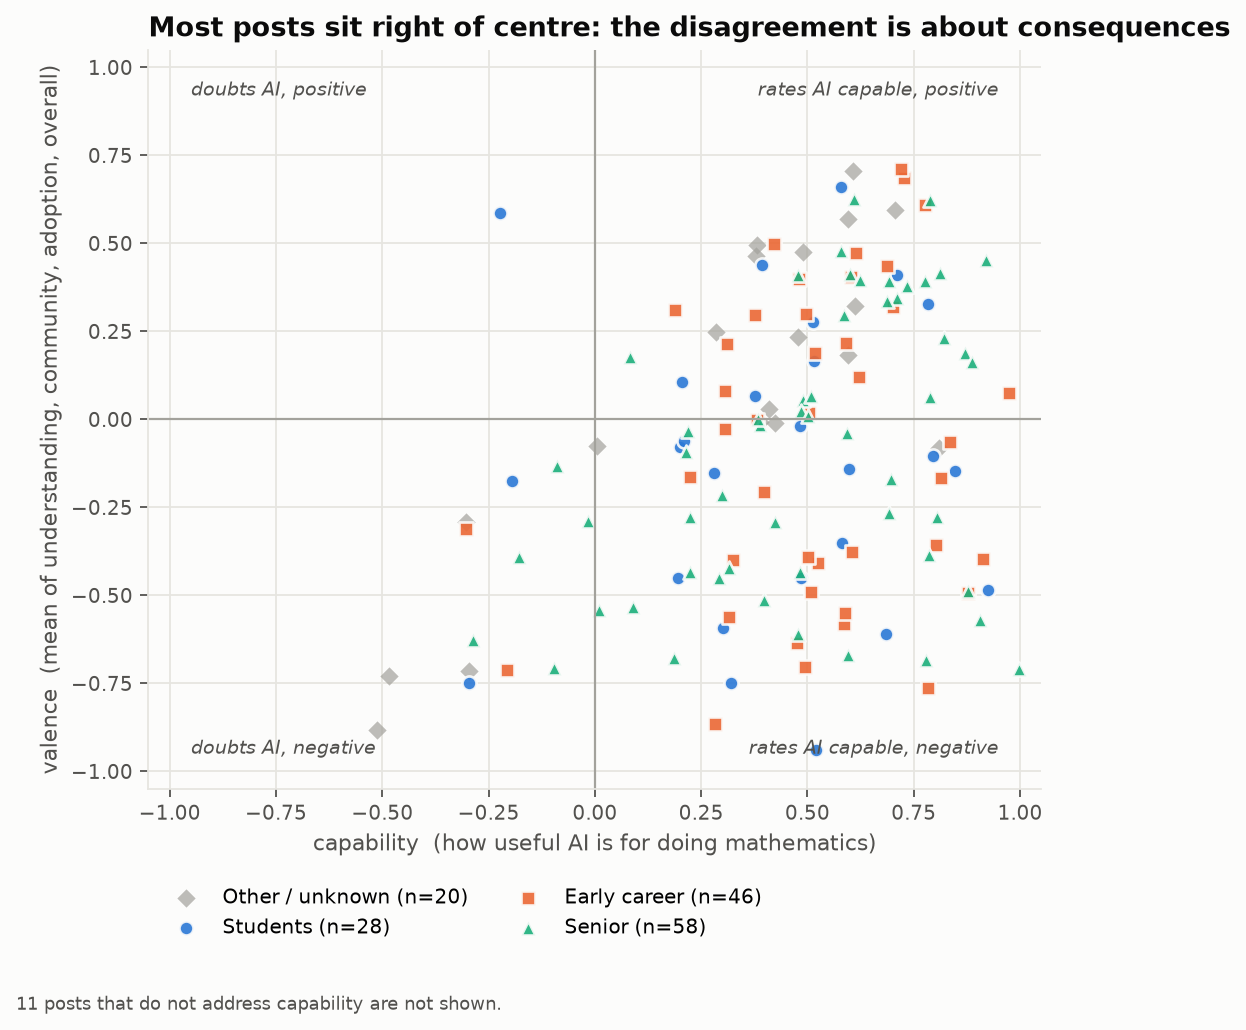
\includegraphics[height=6.1cm]{../figures/04_capability_vs_valence.png}};
    % the site: logo, name, tagline, one-line description (About page and our crawl)
    \node[anchor=north west, inner sep=0pt] (logo) at (8.1,0)
      {
\includegraphics[height=1.0cm]{images/proofs_and_prompts_logo.png}};
    \node[anchor=north west, inner sep=0pt, font=\sffamily\small\bfseries, text=black!85]
      at ([xshift=0.25cm, yshift=-0.12cm]logo.north east) {Proofs and Prompts};
    \node[anchor=north west, inner sep=0pt, font=\rmfamily\itshape\scriptsize, text=black!60]
      at ([xshift=0.25cm, yshift=-0.6cm]logo.north east) {``Notes from the common room''};
    \node[anchor=north west, text width=6.2cm, align=flush left, inner sep=0pt,
          font=\sffamily\scriptsize, text=black!75] at (8.1,-1.25)
      {A blog by mathematicians, for mathematicians, on how AI is changing their practice.
       171 posts from 151 contributors, Aug--Nov 2026. No party line; it invites PhD students and skeptics.};
    \draw[black!12, line width=0.4pt] (8.1,-2.35) -- (14.3,-2.35);
    \node[anchor=north west, text width=6.2cm, align=flush left, inner sep=0pt,
          font=\sffamily\small] at (8.1,-2.55) {%
      {\color{black!55}\scriptsize 152 essays, each scored by an LLM}\par\smallskip
      {\fontsize{20}{22}\selectfont\bfseries\color{tlBlue}89\%}\par
      rate AI as capable of doing mathematics\par\medskip
      {\fontsize{20}{22}\selectfont\bfseries\color{tlOrange}49\%}\par
      view AI as a negative force overall
      };
  \end{tikzpicture}
  \slidesources{proofsandprompts.com, About page (logo by Radhika Gupta); posts crawled 7 Aug--9 Nov 2026 \textbullet{} Proofs \& Prompts corpus, scored with Claude; analysis set of 152 posts, 141 addressing capability. Self-selected essays: an illustration, not a survey}
\end{frame}

% [1 min] The three clusters and the words that distinguish them. The method
% is kept off the slide (removed 2026-11-10); it is here for questions.
% Method (cluster.py, reviewed 2026-11-10): an LLM embeds each post in an
% interpretable semantic space (rubric.py: seven scored dimensions). Clustering
% uses two coordinates of that embedding, capability and valence (mean of
% understanding, community, adoption, overall), standardised, with k-means (k=3, 141 posts; silhouette 0.43, bootstrap ARI median 0.91).
% Cluster names come from a rule on the centres (name_cluster: capability >= 0.4
% -> "capable", else "doubted"; valence > 0.15 positive, < -0.15 negative). The
% "doubted" centre sits at capability +0.04, i.e. neutral rather than doubting.
% Word clouds are computed afterwards from the raw text: per-cluster log-odds of a term appearing in a post
% (z >= 2, >= 5 posts), with a hand-curated list of generic words removed.
\begin{frame}{Proofs and Prompts: What Each Cluster Writes About}
  \centering
  \begin{tikzpicture}[x=1cm, y=1cm]
    \useasboundingbox (0,0) rectangle (14.3,-5.95);
    % clusters in the score plane (figure is 0.872 wide per unit height: ~5.1 cm here);
    % cluster names, sizes and centres are labelled inside the figure
    \node[collagecard, anchor=north west] at (0,0)
      {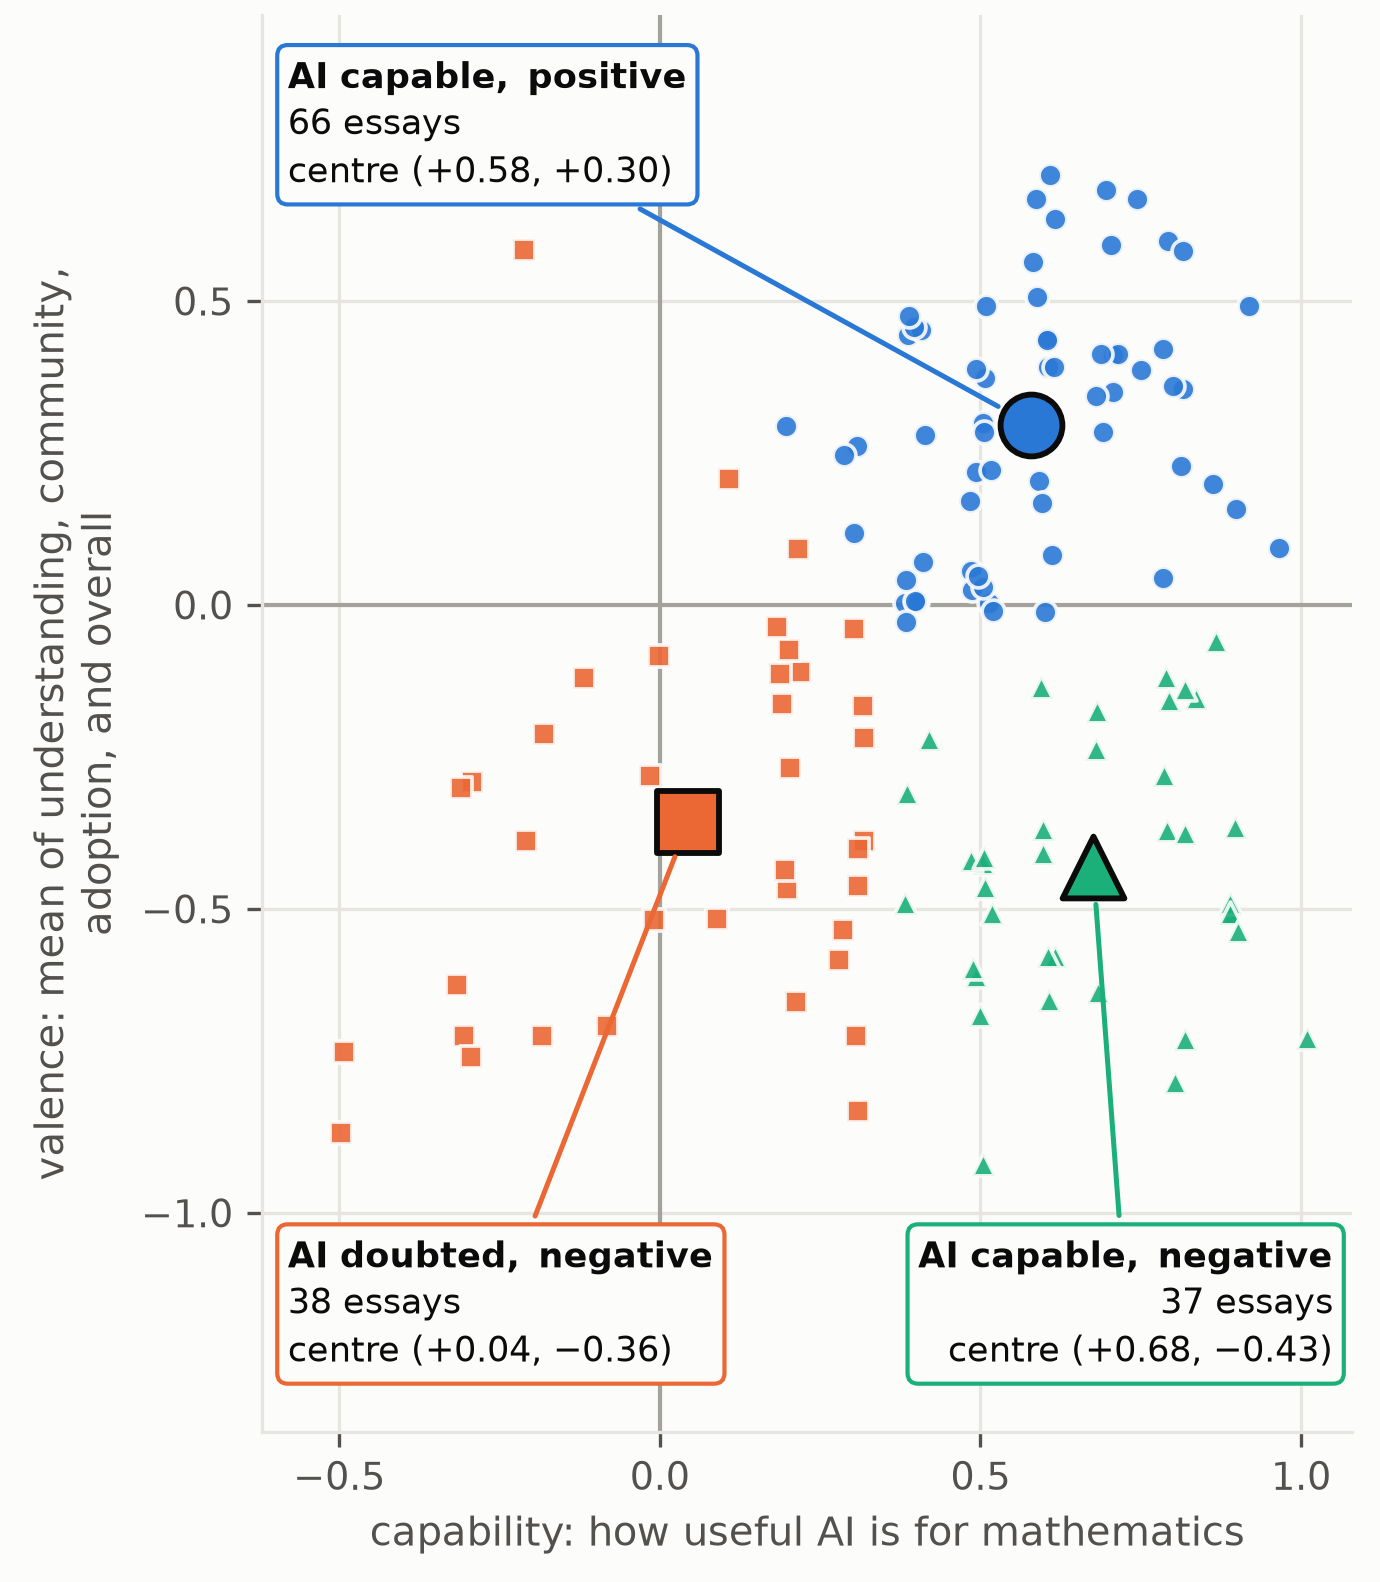
\includegraphics[height=5.85cm]{../figures/08_clusters.png}};
    % word clouds, one per cluster, stacked top to bottom in the same colours (2:3 figure)
    \node[collagecard, anchor=north east] at (14.3,0)
      {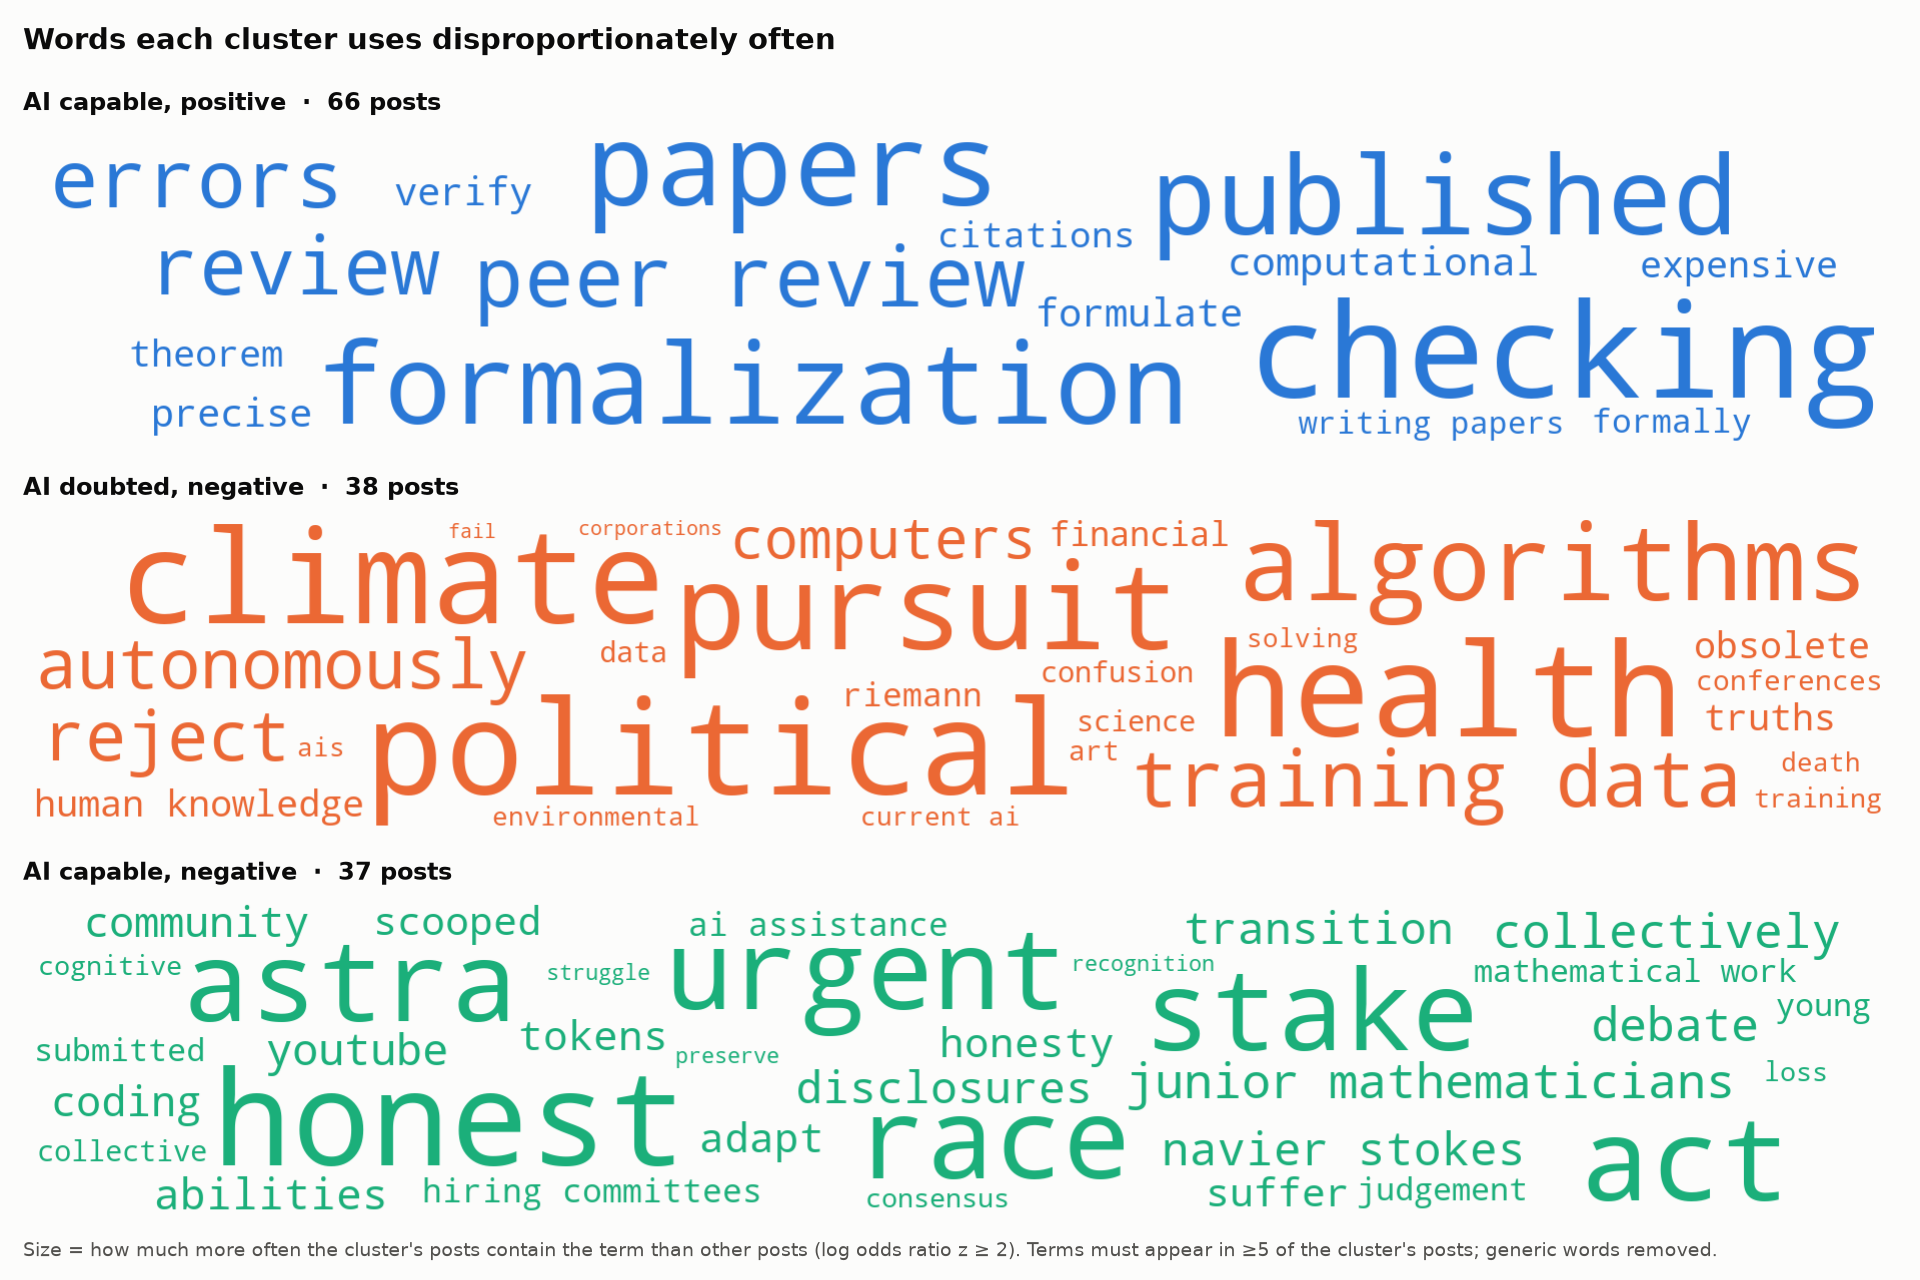
\includegraphics[height=5.85cm]{../figures/09_wordclouds.png}};
  \end{tikzpicture}
  \slidesources{Proofs \& Prompts corpus; scores from Claude (rubric.py); clustering and word statistics from cluster.py. Self-selected essays: an illustration, not a survey}
\end{frame}
